%% Congresso Brasileiro de Fisica Medica (CBFM)
%% 
%% Nome: Rodrigo de Barros Vimieiro
%% E-mail: rodrigo.vimieiro@gmail.com
%%
%% Universidade de São Paulo - São Carlos
%% Laboratório de Visão Computacional - LAVI
%%
%% Data: 10/04/2019

% vvvvvvvvvvvvvvvvvvvvv
% Compiled with XeLateX
% ^^^^^^^^^^^^^^^^^^^^^

\documentclass[10pt,twoside,twocolumn]{article}
\bibliographystyle{vancouver}

%%%%%%%%%%%%%%%%%%%% Packages %%%%%%%%%%%%%%%%%%%%

\usepackage[utf8]{inputenc}
\usepackage{fontspec}
\setmainfont{Arial}
\usepackage{fancyhdr}
\renewcommand{\footrulewidth}{0.4pt}
\usepackage[labelsep=endash]{caption}
\usepackage[font=small]{caption}
\usepackage{titlesec}
\titleformat*{\section}{\normalsize\bfseries}
\titleformat*{\subsection}{\normalsize\itshape}
\titlelabel{\thetitle.\quad}
\usepackage[portuguese]{babel}
\usepackage{graphicx}
\usepackage{amsmath}
\usepackage{amssymb}
\usepackage{xcolor}
\usepackage{geometry}
 \geometry{
 a4paper,
 top = 3cm,
 headsep=2cm,
 width=17.2cm,
 inner=2cm,
 outer=1.8cm,
 }
 
 %%%%%%%%%%%%%%%%%%%% Color notations %%%%%%%%%%%%%%%%%%%%
 
 \newcommand{\rv}[1]{{\textcolor[rgb]{.5,.7,.15}{\small[\textbf{Rodrigo}: #1]}}}	%(Rodrigo)
\newcommand{\lb}[1]{{\textcolor[rgb]{.5,.0,.0}{\small[\textbf{Lucas}: #1]}}}	%(Lucas)
\newcommand{\RV}[2]{{\textcolor[rgb]{.5,.7,.15}{\uwave{#1 }\small[\sout{#2}]}}} %(Rodrigo)
\newcommand{\LB}[2]{{\textcolor[rgb]{.5,.0,.0}{\uwave{#1 }\small[\sout{#2}]}}} %(Lucas)
\newcommand{\rb}[1]{{\textcolor[rgb]{.1,.1,.5}{\small[\textbf{Renann}: #1]}}}	%(Renann)
 
 
 %%%%%%%%%%%%%%%%%%%% Begin document %%%%%%%%%%%%%%%%%%%%
 
\begin{document}


%%%%%%%%%%%% Headers and footers %%%%%%%%%%%% 

\pagestyle{fancy}
\fancyhf{}
\fancyfoot{}
\lhead{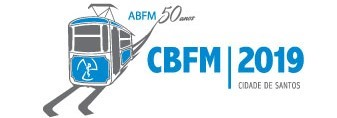
\includegraphics[height=1.8cm]{heads/CBFM_head.jpg}}
\rhead{
        \large \textbf{XXIV Congresso Brasileiro de Física Médica\\
        21 a 24 de Agosto de 2019\\
        Santos}
}
\rfoot{\small \thepage}
\lfoot{\small \textit{Associação Brasileira de Física Médica}\space \textregistered}

%%%%%%%%%%%%%%%%%%%%%%%%%%%%%%%%%%%%%%%%%%%%%%%%%%%%%%%%%%%%%%%%%%%%%%%%%
%                                                                       %
%%%%%%%%%%%%%%%%%%%%%%%%%%%%%%%%%%%%%%%%%%%%%%%%%%%%%%%%%%%%%%%%%%%%%%%%%

%%%%%%%%%%%% Headers informations %%%%%%%%%%%%

\twocolumn[
  \begin{@twocolumnfalse}
  
    \begin{flushright}

        \Large{
        \textbf{Assessment of dose reduction simulation in digital breast tomosynthesis system with amorphous silicon (a-Si) detector}
        }
        
        \large{
        Information for Authors for Full Paper Submission\\
        to the Congresso Brasileiro de F\'{i}sica M\'{e}dica
        }
        
        \vspace{\baselineskip}
        
        Primeiro A. Autor$^{1}$, Segundo B. Co-autor$^{2}$, \'{U}ltimo C. Co-autor$^{3}$\\
        
       \vspace{\baselineskip}
       
       \normalsize{
        
        $^{1}$\textit{Institui\c{c}\~{a}o/Afilia\c{c}\~{a}o, Cidade, Pa\'{i}s}
        
        $^{2}$\textit{Divis\~{a}o/Servi\c{c}o/Departamento, Instituto/Hospital/Universidade, Cidade, Pa\'{i}s}
        
        $^{3}$\textit{Servi\c{c}o/Departamento, Hospital/Universidade, Cidade, Pa\'{i}s}
        
        }

    \end{flushright}

%%%%%%%%%%%%%%%%%%%%%%%%%%%%%%%%%%%%%%%%%%%%%%%%%%%%%%%%%%%%%%%%%%%%%%%%%
%                                                                       %
%%%%%%%%%%%%%%%%%%%%%%%%%%%%%%%%%%%%%%%%%%%%%%%%%%%%%%%%%%%%%%%%%%%%%%%%%

%%%%%%%%%%%% Resumo %%%%%%%%%%%%

\textbf{Resumo}

Este modelo apresenta as instruções para a submissão de artigos completos ao Congresso Brasileiro de Física Médica (CBFM). Os artigos devem ser submetidos eletronicamente pelo website da CBFM. Serão aceitos artigos em português, espanhol e inglês, com, no mínimo, 4 (quatro) páginas, e no máximo, 10 (dez) páginas. O resumo/abstract deve conter, no mínimo 150 e no máximo, 300 palavras. Sempre que o artigo for escrito em língua estrangeira, um resumo em português é exigido. Devem ser listados, abaixo do resumo, de 3 (três) até 6 (seis) unitermos/palavras-chave, preferencialmente de acordo com os Descritores em Ciências da Saúde (DeCS) ou com o Medical Subject Headings (MeSH) da National Library of Medicine (http://www.nlm.nih.gov), ou com o Physics and Astronomy Classification Scheme (PACS - http://www.aip.org/pacs/index.html), separados por ponto e vírgula. As referências devem ser numeradas e citadas de acordo com a ordem de aparecimento no artigo. As referências devem ser escritas ao estilo Vancouver.

\textbf{Palavras-chave}: f\'{i}sica m\'{e}dica; medicina nuclear; radioterapia; radiologia; prote\c{c}\~{a}o radiol\'{o}gica.\\


%%%%%%%%%%%% Abstract %%%%%%%%%%%%

\textbf{\textit{Abstract}}

\textit{This model presents the instructions for submitting full papers to the Brazilian Congress of Medical Physics (CBFM). The papers must be submitted electronically in CBFM website. Papers will be accepted in Portuguese, Spanish and English, with a minimum of 4 (four) pages and a maximum of 10 (ten) pages. The abstract should contain a minimum of 150 and a maximum of 300 words. Whenever the article is written in a foreign language, a summary in Portuguese is mandatory. Three (3) to six (6) keywords should be listed below the abstracts, preferably in accordance with the Health Sciences Descriptors (DeCS) or the Medical Subject Headings (MeSH) of the National Library of Medicine (http://www.nlm.nih.gov), or the Physics and Astronomy Classification Scheme (PACS - http://www.aip.org/pacs/index.html), separated by a semicolon. References should be numbered and quoted according to the order of appearance in the article. The references must de written in the Vancouver style.}

\textbf{Keywords}\textit{: medical physics; nuclear medicine; radiation oncology; radiology; radiation protection.} 

\vspace{\baselineskip}
    \end{@twocolumnfalse}
 ]
 
%%%%%%%%%%%%%%%%%%%%%%%%%%%%%%%%%%%%%%%%%%%%%%%%%%%%%%%%%%%%%%%%%%%%%%%%%
%                                                                       %
%%%%%%%%%%%%%%%%%%%%%%%%%%%%%%%%%%%%%%%%%%%%%%%%%%%%%%%%%%%%%%%%%%%%%%%%%
 
%%%%%%%%%%%% Introduction %%%%%%%%%%%% 
 
\section{Introduction}

O Congresso Brasileiro de Física Médica (CBFM) é um congresso anual, promovido pela Associação Brasileira de Física Médica (ABFM). 
Dois tipos de trabalhos podem ser submetidos ao CBFM: artigo completo ou resumo expandido. O  artigo completo caracteriza-se por um artigo de caráter técnico-científico, que possui um objetivo bem definido, materiais e métodos bem delineados e resultados que podem ser comparados com outros trabalhos da literatura. O resumo expandido destina-se a trabalhos em andamento, que possuem objetivos e materiais/métodos bem definidos, mas que podem ter apenas resultados preliminares ou tratarem de uma comunicação técnica.

Os artigos devem ser submetidos na sua versão final, eletronicamente, pelo website da CBFM, em formato Adobe Acrobat (*.pdf).
O artigo deve ser estruturado em seções numeradas: Introdução, que traz o contexto do trabalho, assim como seu objetivo; Materiais e Métodos, nos quais se descrevem os materiais utilizados no trabalho e os métodos utilizados; Resultados, contendo dados numéricos ou categóricos, gráficos e tabelas; Discussão, no qual os autores explicam seus resultados, dialogando com a literatura pertinente; e as Conclusões.
O objetivo deste artigo é apresentar os detalhes da estrutura e formatação de um artigo completo a ser submetido para o CBFM.

Serão aceitos artigos em português, espanhol e inglês, com no máximo, 10 (dez) páginas e, no mínimo, 4 (quatro) páginas, incluindo Ilustrações, Tabelas e Referências. O corpo do artigo deve ser escrito utilizando fonte Arial, tamanho 10. O espaçamento no corpo do texto deve ser no padrão simples e o alinhamento do texto deve ser justificado em ambos os lados. Não inserir linhas em branco entre parágrafos, a não ser antes e depois das ilustrações e tabelas. Para artigos redigidos em português ou espanhol, os termos citados no texto em inglês devem estar no formato itálico.
O artigo deve ser redigido em formato de papel tipo A4 (21,0 x 29,7 cm), com margens e espaçamentos conforme o modelo. O layout de página deve obedecer à formatação de dupla coluna com largura e espaçamento, conforme o modelo, com exceção à seção que contém título/autoria e resumo/abstract, na qual uma única coluna é empregada.
Os artigos originais devem ser escritos preferencialmente conforme as seguintes divisões de seções: Introdução, Materiais e Métodos, Resultados, Discussão, Conclusões, Agradecimentos (opcional) e Referências. Os títulos das seções devem estar em negrito e devem ser numerados em algarismo arábico. As seções Agradecimentos e Referências não devem ser numeradas. Outros títulos das seções podem ser empregados, mas seu conteúdo deve abordar todos os aspectos de um artigo científico original. Nas subseções utilizar, no máximo, dois níveis, conforme formatação apresentada a seguir.



\section{Theoretical Background}

\subsection{Noise model}


\begin{equation}
\label{eq.Eq1}
 y^{o}(i,j) = y(i,j) + \sigma(y(i,j)) \, \xi(0,1) + \tau,
\end{equation}


\begin{enumerate}
    \item Linearization,
    \item Quantum noise injection,
    \item Signal scaling,
    \item Electronic noise injection,
    \item Offset injection.
\end{enumerate}



\section{Materials \& Methods}



\begin{table}[ht]
\caption{DBT system characteristics \cite{vedantham2015digital}.}
	\label{tab:tab1}
   	\centering
% 	\footnotesize
	\begin{tabular}{l|c}
		\textbf{Characteristic}                                       &        \textbf{Colocar algo aq}              \\
		[1pt]
		\hline
        \rule[-0.5ex]{-3pt}{1ex}
		Detector type                 &         CsI:Tl (Indirect)                               \\ \hline
       	\rule[-0.5ex]{-3pt}{1ex}
		Manufacturer &    General Electric    \\ \hline
		\rule[-0.5ex]{-3pt}{1ex}
		Model &    Senographe Essential    \\ \hline
		\rule[-0.5ex]{-3pt}{1ex}
		Projection number              &                9                                               \\ \hline
		\rule[-0.5ex]{-3pt}{1ex}
		Tube angle span                &           $25^{\circ}$          		                          \\ \hline
		\rule[-0.5ex]{-3pt}{1ex}
		Detector angle span           &          Stationary                                  \\ \hline
		\rule[-0.5ex]{-3pt}{1ex}
		Tube movement                &     Step-and-shoot                              \\ \hline
		\rule[-0.5ex]{-3pt}{1ex}
		Pixel size        &            100$\mu$m                                \\ \hline
	\end{tabular}
\end{table}

\section{Results \& Discussion}


\begin{figure}[!ht]
    \caption{.}
	\label{fig:img1}
	\begin{center}
		\includegraphics[scale=.56]{imgs/Machine1/with36/SNR.png}
	\end{center}
\end{figure}




\section{Conclusion}


\section*{Acknowledgments}



\bibliography{bibliography}

\end{document}
